\chapter{Resultados}
\label{cap:principal}

Este capítulo consiste no núcleo principal do trabalho, contendo todas as informações e dados coletados.
Este é um dos itens mais importantes do trabalho. Nele os resultados obtidos são comparados, analisados e discutidos, fornecendo elementos para o capítulo de Conclusões.
O nome do capítulo pode e deve ser alterado para melhor caracterizar o conteúdo conforme o tema estudado.
Além disso, o conteúdo pode ser dividido em mais capítulos a critério do autor e de seus orientadores.

\begin{figure}[!ht]
    \begin{minipage}{.5\textwidth}
        \centering
        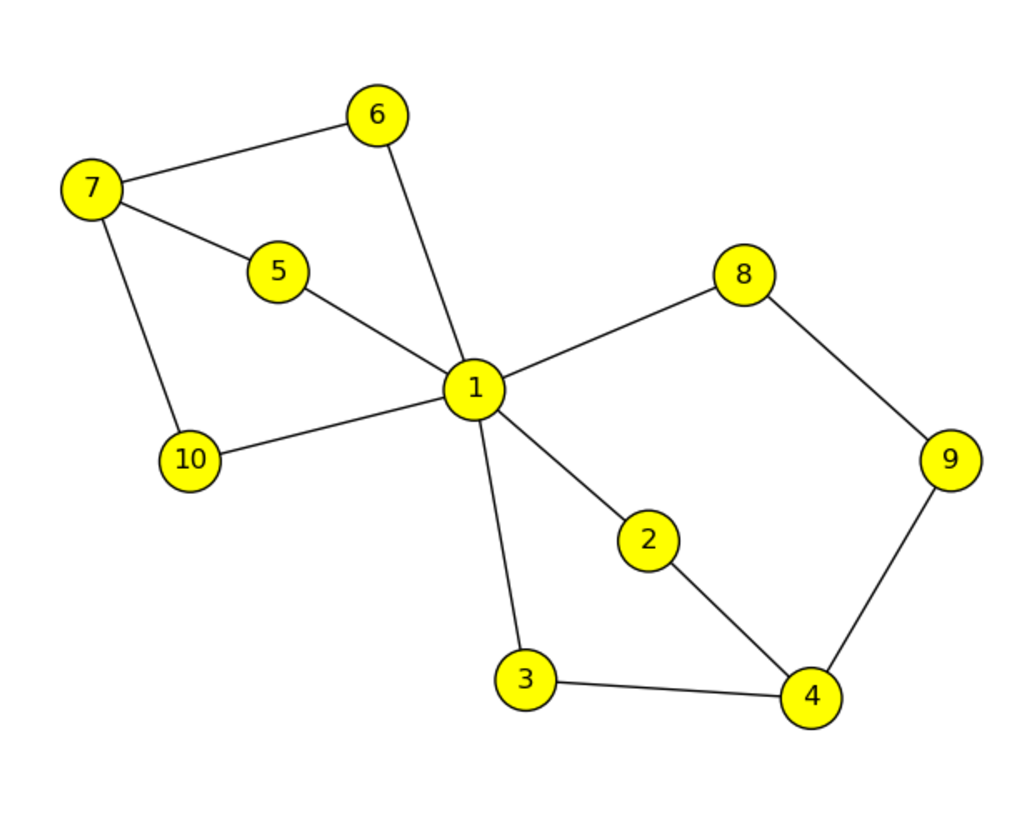
\includegraphics[width=1.0\textwidth]{figs/artigo1.eps}
        \footnotesize\centerline{(a)}\medskip
    \end{minipage}
    \hfill
    \begin{minipage}{.5\textwidth}
        \centering
        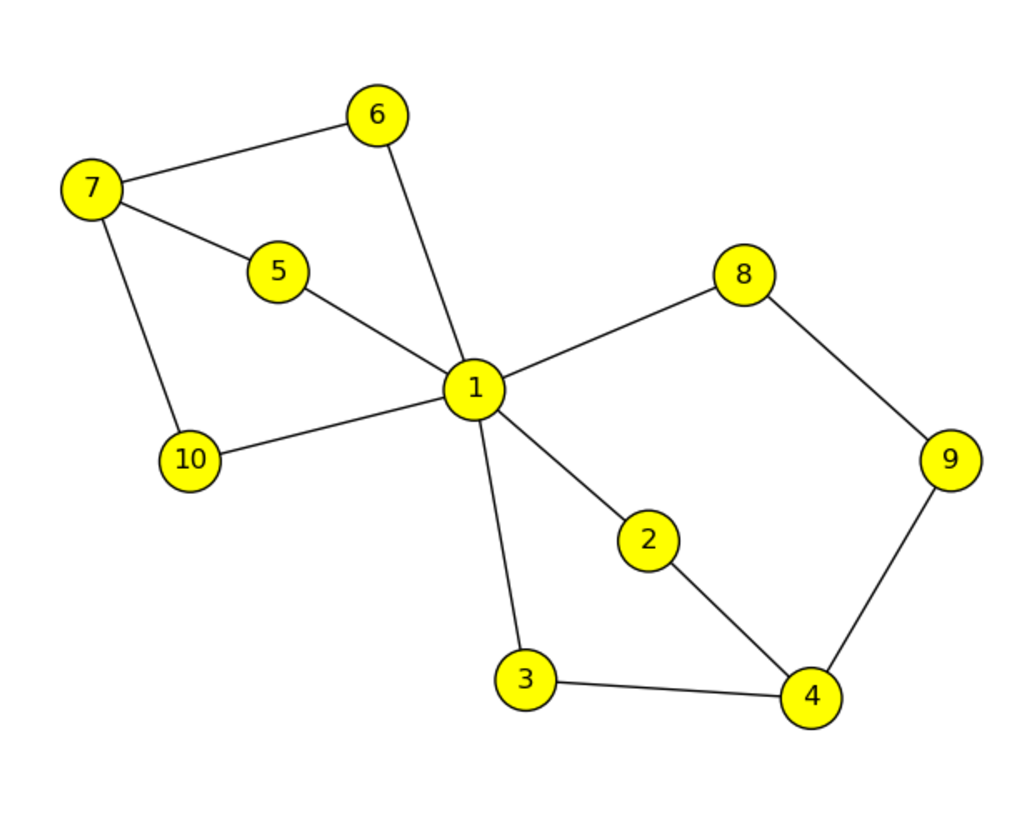
\includegraphics[width=1.0\textwidth]{figs/artigo1.eps}
        \footnotesize\centerline{(b)}\medskip
    \end{minipage}
    \caption{Exemplo de uma figura com duas imagens. \textbf{(a)} descrição da primeira imagem \textbf{(b)} descrição da segunda imagem.}
    \label{fig: phantom IV spectrogram and background noise}
\end{figure}